% #702 | Archive/2024/TOAN_11_XE/TOAN_11_XE/data4/11C5/KNTT-5.1.tex | mã gốc 1C3B1-5
\begin{vd}%[1C3B1-5]
	Cho cấp số nhân $(u_n)$, với $u_1=1$ và công bội $q=\dfrac{1}{2}$.
	\begin{enumEX}{1}
		\item So sánh $\left|q\right|$ với $1$.
		\item Tính $S_n=u_1+u_2+\cdots+u_n$ từ đó hãy tính $\lim S_n$.
	\end{enumEX}
	\loigiai{
		\begin{enumerate}
			\item Ta có $\left|q\right|=\left|\dfrac{1}{2}\right|=\dfrac{1}{2}<1$.
			\item Ta có $S_n=\dfrac{u_1\left(1-q^n\right)}{1-q}=\dfrac{1\cdot\left[1-\left(\dfrac{1}{2}\right)^n\right]}{1-\dfrac{1}{2}}=2\cdot\left(1-\dfrac{1}{2^n}\right)=2-\dfrac{1}{2^{n-1}}$.\\
			Khi đó $\lim S_n=\lim \left(2-\dfrac{1}{2^{n-1}}\right)=2$.
		\end{enumerate}
	}
\end{vd}

% #703 | Archive/2024/TOAN_11_XE/TOAN_11_XE/data4/11C5/KNTT-5.1.tex | mã gốc 1C3Y1-5
\begin{vd}%[1C3Y1-5]
	Tính tổng $T=1+\dfrac{1}{3}+\dfrac{1}{3^2}+\ldots+\dfrac{1}{3^n}+\ldots$
	\loigiai{
		Các số hạn của tổng lập thành câp số nhân $(u_n)$, có $u_1=1$, $q=\dfrac{1}{3}$ nên\\ $$T=1+\dfrac{1}{3}+\dfrac{1}{3^2}+\ldots+\dfrac{1}{3^n}+\ldots=\dfrac{1}{1-\dfrac{1}{3}}=\dfrac{2}{3}\cdot$$
	}
\end{vd}

% #704 | Archive/2024/TOAN_11_XE/TOAN_11_XE/data4/11C5/KNTT-5.1.tex | mã gốc 1C3B1-5
\begin{vd}%[1C3B1-5]
	Biểu diễn số thập phân vô hạn tuần hoàn $2{,}222 \ldots$ dưới dạng phân số.
	\loigiai{
		Ta có $2{,}222 \ldots=2+0{,}2+0{,}02+0{,}002+\ldots=2+2 \cdot 10^{-1}+2 \cdot 10^{-2}+2 \cdot 10^{-3}+\ldots$.\\
		Đây là tổng của cấp số nhân lùi vô hạn với $u_{1}=2, q=10^{-1}$ nên
		$$
		2{,}222 \ldots=\dfrac{u_{1}}{1-q}=\dfrac{2}{1-\dfrac{1}{10}}=\dfrac{20}{9}.
		$$
	}
\end{vd}

% #705 | Archive/2024/TOAN_11_XE/TOAN_11_XE/data4/11C5/KNTT-5.1.tex | mã gốc 1C3B1-5
\begin{vd}%[1C3B1-5]
	Biểu diễn số thập phân vô hạn tuần hoàn $0,(3)$ dưới dạng phân số.
	\loigiai{
		Ta có  $0,(3)=\dfrac{3}{10}+\dfrac{3}{10^2}+\ldots+\dfrac{3}{10^n}+\ldots=\dfrac{\dfrac{3}{10}}{1-\dfrac{1}{10}}=\dfrac{1}{3}\cdot$
	}
\end{vd}

% #706 | Archive/2024/TOAN_11_XE/TOAN_11_XE/data4/11C5/KNTT-5.1.tex | mã gốc 1C3K1-6
\begin{vd}%[1C3K1-6]
	\immini{Từ hình vuông có độ dài cạnh bằng $1$, người ta nối các trung điểm của cạnh hình vuông để tạo ra hình vuông mới như hình bên. Tiếp tục quá trình này đến vô hạn.
		\begin{enumEX}{1}
			\item Tính diện tích $S_n$ của hình vuông được tạo thành từ bước thứ $n$.
			\item Tính tổng diện tích của tất cả các hình vuông được tạo thành.
	\end{enumEX}}	
	{
		\begin{tikzpicture}[scale=0.6, font=\footnotesize,>=stealth]
			\def\canhAD{6};
			\coordinate (D) at (0,0);
			\coordinate (A) at ($(D)+(90:\canhAD)$);
			\coordinate (C) at ($(D)+(0:\canhAD)$);
			\coordinate (B) at ($(A)+(0:\canhAD)$);
			\coordinate (E) at ($(A)!0.5!(B)$);
			\coordinate (F) at ($(B)!0.5!(C)$);
			\coordinate (G) at ($(C)!0.5!(D)$);
			\coordinate (H) at ($(D)!0.5!(A)$);
			\coordinate (K) at ($(E)!0.5!(F)$);
			\coordinate (L) at ($(F)!0.5!(G)$);
			\coordinate (M) at ($(G)!0.5!(H)$);
			\coordinate (J) at ($(H)!0.5!(E)$);
			\coordinate (I) at ($(E)!0.5!(G)$);
			\coordinate (X) at ($(J)!0.5!(K)$);
			\coordinate (Y) at ($(K)!0.5!(L)$);
			\coordinate (T) at ($(L)!0.5!(M)$);
			\coordinate (Q) at ($(M)!0.5!(J)$);
			\draw(A) rectangle (C)(E)--(F)--(G)--(H)--cycle (J)--(K)--(L)--(M)--cycle (X)--(Y)--(T)--(Q)--cycle;
			\draw [>=stealth,|<->|] ([shift=({0,-0.4})]D)--([shift=({0,-0.4})]C) node [midway,below]{$1$};
			
			%			\foreach \x/\y in {A/90,D/-90,C/-90,B/90,E/90,G/-90,H/180,F/0,K/90,L/-90,M/-90,J/90,I/-110}{\fill (\x) circle(1pt) ($(\x)+(\y:0.3cm)$) node{$\x$};}
		\end{tikzpicture}
	}
	
	\loigiai{
		\begin{enumerate}
			\item Từ giả thiết suy ra diện tích hình vuông sau bằng $\dfrac{1}{2}$ diện tích hình vuông trước.\\ 
			Khi đó diện tích của các hình vuông tạo thành một cấp số nhân lùi vô hạn với số hạng đầu $S_1=1$ và công bội $q=\dfrac{1}{2}$.\\
			Diện tích $S_n$ của hình vuông được tạo thành từ bước thứ $n$ là $S_n=S_1\cdot q^{n-1}=\left(\dfrac{1}{2}\right)^{n-1}$.
			\item Tổng diện tích của tất cả các hình vuông được tạo thành là:\\
			$$S=\dfrac{u_1}{1-q}=\dfrac{1}{1-\dfrac{1}{2}}=2.$$
		\end{enumerate}
	}
\end{vd}

% #707 | Archive/2024/TOAN_11_XE/TOAN_11_XE/data4/11C5/KNTT-5.1.tex | mã gốc 1C3K1-6
\begin{vd}%[1C3K1-6]
	Có $1$ kg chất phóng xạ độc hại. Biết rằng, cứ sau một khoảng thời gian $T=24000$ năm thì một nửa số chất phóng xạ này bị phân rã thành chất khác không độc hại đối với sức khỏe của con người ($T$ được gọi là \textit{chu kì bán rã}).
	\begin{flushright}
		(\textit{Nguồn: Đại số và giải tích 11, NXB GD Việt Nam, 2021})
	\end{flushright}
	Gọi $u_n$ là khối lượng chất phóng xạ còn lại sau chu kì thứ $n$.
	\begin{enumerate}
		\item  Tìm số hạng tổng quát $u_n$ của dãy số $(u_n)$.
		\item  Chứng minh rằng $(u_n)$ có giới hạn là $0$.
		\item  Từ kết quả câu $2$, chứng tỏ rằng sau một số năm nào đó khối lượng phóng xạ đã cho ban đầu không còn độc hại với con người, biết rằng chất phóng xạ này sẽ không độc hại nữa nếu khối lượng chất phóng xạ còn lại bé hơn $10^{-6}$ g.
	\end{enumerate}
	\loigiai{
		\begin{enumerate}
			\item  Khối lượng chất phóng xạ còn lại sau chu kì bán rã thứ $1$ là $u_1=\dfrac{1}{2}\cdot 1=1$ kg.\\
			Khối lượng chất phóng xạ còn lại sau chu kì bán rã thứ $2$ là $u_2=\dfrac{1}{2}\cdot u_1=\dfrac{1}{2}\cdot \dfrac{1}{2}=\dfrac{1}{2^2}$ kg.\\
			Khối lượng chất phóng xạ còn lại sau chu kì bán rã thứ $3$ là $u_3=\dfrac{1}{2}\cdot u_2=\dfrac{1}{2}\cdot \dfrac{1}{4}=\dfrac{1}{2^3}$ kg.\\
			Khối lượng chất phóng xạ còn lại sau chu kì bán rã thứ $n$ là $u_n=\dfrac{1}{2^n}$ kg.\\
			\item $\lim u_n=\lim \dfrac{1}{2^n}=\lim\left(\dfrac{1}{2}\right)^n=0$.
			\item Chất phóng xạ sẽ không độc hại nữa nếu khối lượng chất phóng xạ còn lại bé hơn $10^{-6}~\mathrm{g}=10^{-9}$ kg
			$$\Leftrightarrow u_n<10^{-9}\Leftrightarrow\dfrac{1}{2^n}<10^{-9}\Leftrightarrow 2^n>10^9\Leftrightarrow n\geq 30.$$
			Vậy sau ít nhất $30$ chu kì bằng $30\cdot 24000=720000$ năm thì khối lượng phóng xạ đã cho ban đầu không còn độc hại với con người nữa.
		\end{enumerate}
	}
\end{vd}

% #708 | Archive/2024/TOAN_11_XE/TOAN_11_XE/data4/11C5/KNTT-5.1.tex | mã gốc 1C3G1-6
\begin{vd}%[1C3G1-6]
	Gọi $C$ là nữa đường tròn đường kính $AB=2R$.\\
	$C_1$ là đường gồm hai nửa đường tròn đường kính $\dfrac{AB}{2}$,\\
	$C_2$ là đường gồm bốn nửa đường tròn đường kính $\dfrac{AB}{4},\cdots$\\
	$C_n$ là đường gồm $2^n$ nửa đường tròn đường kính $\dfrac{AB}{2^n},\cdots$
	\immini{	Gọi $p_n$ là độ dài của $C_n$, $S_n$ là diện tích hình phẳng giới hạn bởi $C_n$ và đoạn thẳng $AB$.
		\begin{enumEX}{1}
			\item Tính $p_n$, $S_n$.
			\item Tính giới hạn của các dãy số $(p_n)$ và $(S_n)$.
		\end{enumEX}
	}{
		\begin{tikzpicture}[declare function={r=3;}]
			\path
			(0,0) coordinate (O)
			(0:r) coordinate (A)
			(180:r) coordinate (B)
			($(A)!.5!(O)$) coordinate (M)
			($(B)!.5!(O)$) coordinate (N)
			($(B)!.5!(N)$) coordinate (I)
			($(N)!.5!(O)$) coordinate (J)
			($(O)!.5!(M)$) coordinate (K)
			($(M)!.5!(A)$) coordinate (H)
			($(B)!.5!(I)$) coordinate (Q);
			\draw (A) arc(0:180:r) (A) arc(0:180:r/2) (O) arc(0:180:r/2) (A) arc(0:180:r/4) (A) arc(0:180:r/4)(M) arc(0:180:r/4) (O) arc(0:180:r/4) (N) arc(0:180:r/4)
			(A) arc(0:180:r/8) (H) arc(0:180:r/8) (M) arc(0:180:r/8) (K) arc(0:180:r/8) (O) arc(0:180:r/8) (J) arc(0:180:r/8) (N) arc(0:180:r/8) (I) arc(0:180:r/8);
			\draw (A)--(B);
			\path 
			($(O)+(90:0.9*r)$) node{$C$}
			($(N)+(90:0.4*r)$) node[scale=0.8]{$C_1$}
			($(I)+(90:0.18*r)$) node[scale=0.7]{$C_2$}
			($(Q)+(90:0.06*r)$) node[scale=0.6]{$C_3$};
			\foreach \x/\y in {A/-90, B/-90}{\fill (\x) circle(1pt) ($(\x)+(\y:0.3cm)$) node{$\x$};}
		\end{tikzpicture}
	}
	
	\loigiai{
		\begin{enumerate}
			\item Ta có  
			\begin{eqnarray*}
				p_n&=&2^n \cdot \pi r=2^n\cdot\pi \cdot \dfrac{AB}{2\cdot2^n}\\
				&=&\dfrac{\pi AB}{2}\\
				&=&\dfrac{\pi \cdot 2R}{2}\\
				&=&\pi R.
			\end{eqnarray*}
			\begin{eqnarray*}
				S_n&=&2^n \cdot \dfrac{1}{2}\pi r^2\\
				&=&2^n \cdot \dfrac{1}{2}\pi \left(\dfrac{AB}{2\cdot2^n}\right)^2\\
				&=&2^n \cdot \dfrac{1}{2}\pi \left(\dfrac{2R}{2\cdot2^n}\right)^2\\
				&=&2^n \cdot \dfrac{1}{2}\pi \dfrac{R^2}{(2^n)^2}\\
				&=&\dfrac{\pi R^2}{2^{n+1}}.	
			\end{eqnarray*}			
			\item $\lim p_n=\lim \left(\pi R\right) = \pi R$.\\
			$\lim S_n=\lim \dfrac{\pi R^2}{2^{n+1}}=0$ (Vì $\lim \left(\pi R^2\right)=\pi R^2$ và $\lim 2^{n+1}=+\infty$).
		\end{enumerate}
	}
\end{vd}

% #711 | Archive/2024/TOAN_11_XE/TOAN_11_XE/data4/11C5/KNTT-5.1.tex | mã gốc 1C3B1-5
\begin{bt}%[TeX hóa SGK CD]%[Dương Quang]%[1C3B1-5]
	\begin{enumEX}{1}
		\item[] 
		\item Tính tổng cấp số nhân lùi vô hạn $(u_n)$ với $u_1=\dfrac{2}{3}, q=-\dfrac{1}{4}$.
		\item Biểu diễn số thập phân vô hạn tuần hoàn $1,(6)$ dưới dạng phân số.
	\end{enumEX}
	\loigiai{
		\begin{enumerate}
			\item Ta có  $S=\dfrac{u_1}{1-q}=\dfrac{\dfrac{2}{3}}{1-\left(-\dfrac{1}{4}\right)}=\dfrac{8}{15}$.
			\item Ta có  $1,(6)=1+0,(6)=1+\dfrac{6}{10}+\dfrac{6}{10^2}+\cdots+\dfrac{6}{10^n}+\cdots=1+\dfrac{\dfrac{6}{10}}{1-\dfrac{1}{10}}=\dfrac{5}{3}$.
		\end{enumerate}
	}
\end{bt}

% #712 | Archive/2024/TOAN_11_XE/TOAN_11_XE/data4/11C5/KNTT-5.1.tex | mã gốc 1C3K1-6
\begin{bt}%[TeX hóa SGK CD]%[Dương Quang]%[1C3K1-6]
	Có $1$ kg chất phóng xạ độc hại. Biết rằng, cứ sau một khoảng thời gian $T=24000$ năm thì một nửa số chất phóng xạ này bị phân rã thành chất khác không độc hại đối với sức khỏe của con người ($T$ được gọi là \textit{chu kì bán rã}).
	\begin{flushright}
		(\textit{Nguồn: Đại số và giải tích 11, NXB GD Việt Nam, 2021})
	\end{flushright}
	Gọi $u_n$ là khối lượng chất phóng xạ còn lại sau chu kì thứ $n$.
	\begin{enumerate}
		\item  Tìm số hạng tổng quát $u_n$ của dãy số $(u_n)$.
		\item  Chứng minh rằng $(u_n)$ có giới hạn là $0$.
		\item  Từ kết quả câu $b$, chứng tỏ rằng sau một số năm nào đó khối lượng phóng xạ đã cho ban đầu không còn độc hại với con người, biết rằng chất phóng xạ này sẽ không độc hại nữa nếu khối lượng chất phóng xạ còn lại bé hơn $10^{-6}$ g.
	\end{enumerate}
	\loigiai{
		\begin{enumerate}
			\item  Khối lượng chất phóng xạ còn lại sau chu kì bán rã thứ $1$ là $u_1=\dfrac{1}{2}\cdot 1=1$ kg.\\
			Khối lượng chất phóng xạ còn lại sau chu kì bán rã thứ $2$ là $u_2=\dfrac{1}{2}\cdot u_1=\dfrac{1}{2}\cdot \dfrac{1}{2}=\dfrac{1}{2^2}$ kg.\\
			Khối lượng chất phóng xạ còn lại sau chu kì bán rã thứ $3$ là $u_3=\dfrac{1}{2}\cdot u_2=\dfrac{1}{2}\cdot \dfrac{1}{4}=\dfrac{1}{2^3}$ kg.\\
			Khối lượng chất phóng xạ còn lại sau chu kì bán rã thứ $n$ là $u_n=\dfrac{1}{2^n}$ kg.\\
			\item $\lim u_n=\lim \dfrac{1}{2^n}=\lim\left(\dfrac{1}{2}\right)^n=0$.
			\item Chất phóng xạ sẽ không độc hại nữa nếu khối lượng chất phóng xạ còn lại bé hơn $10^{-6}~\mathrm{g}=10^{-9}$ kg
			$$\Leftrightarrow u_n<10^{-9}\Leftrightarrow\dfrac{1}{2^n}<10^{-9}\Leftrightarrow 2^n>10^9\Leftrightarrow n\geq 30.$$
			Vậy sau ít nhất $30$ chu kì bằng $30\cdot 24000=720000$ năm thì khối lượng phóng xạ đã cho ban đầu không còn độc hại với con người nữa.
		\end{enumerate}
	}
\end{bt}

% #713 | Archive/2024/TOAN_11_XE/TOAN_11_XE/data4/11C5/KNTT-5.3.tex | mã gốc 1C3B3-3
\begin{bt}%[Phạm Hoàng Điệp - Dự Án tex  11 mới]%[1C3B3-3]
	Dùng định nghĩa xét tính liên tục của hàm số $ f(x)= 2x^{3}+x+1 $ tại điểm $ x=2 $.
	\loigiai{
		Hàm số trên là hàm sơ cấp nên liên tục trên $ \mathbb{R} $.\\
		%Xét tính liên tục của hàm số tại điểm $ x=2 $.\\
		Ta có $ f(2)=2\cdot 2^{3}+2+1=19 $.\\
		$ \displaystyle\lim\limits_{x\to 2}f(x) =\displaystyle\lim\limits_{x\to 2}\left(2x^{3}+x+1\right)=2\cdot 2^{3}+2+1=19$.\\
		Vậy $ \displaystyle\lim\limits_{x\to 2}f(x)=f(2)=19 $ nên hàm số $ y=2x^{3}+x+1 $ liên tục tại $ x=2 $.
	}
\end{bt}

% #714 | Archive/2024/TOAN_11_XE/TOAN_11_XE/data4/11C5/KNTT-5.3.tex | mã gốc 1C3Y3-4
\begin{bt}%[Phạm Hoàng Điệp - Dự Án tex  11 mới]%[1C3Y3-4]
	Trong các hàm số có đồ thị ở \textit{Hình 15a, 15b, 15c} hàm số nào liên tục trên tập xác định của hàm số đó? Giải thích.
	\begin{longtable}{m{5cm}m{5cm}m{5cm}}
		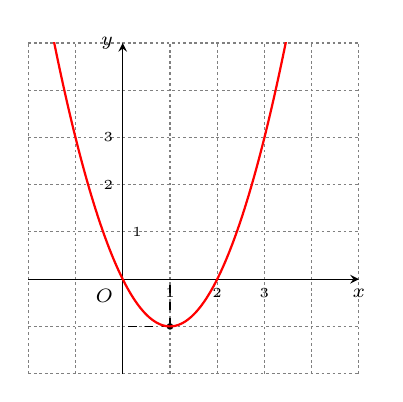
\begin{tikzpicture}[>=stealth,x=1cm,y=1cm,scale=0.6,font=\tiny]
			\def\a{1}
			\def\b{-2}
			\def\c{0}
			\draw[color=gray,dash pattern=on 1pt off 1pt,xstep=1.0cm,ystep=1.0cm] (-2,-2) grid (5,5);
			\draw[->] (-2,0) -- (5,0) node[below] {\scriptsize $x$};
			\draw[->] (0,-2) -- (0,5) node[left] {\scriptsize $y$};
			\draw (0,0)node[below left]{\scriptsize $O$};
			\fill (0,1) node[right]{$1$};
			\fill (0,2) node[left]{$2$};
			\fill (0,3) node[left]{$3$};
			\fill (1,0) node[below]{$1$};
			\fill (2,0) node[below]{$2$};
			\fill (3,0) node[below]{$3$};
			\pgfmathsetmacro\xdinh{-(\b)/2*(\a)}
			\pgfmathsetmacro\ydinh{(4*(\a)*(\c)-(\b)^2)/(4*(\a))}
			\fill[dashed] (\xdinh,\ydinh)circle(2pt) edge (\xdinh,0) edge (0,\ydinh);
			\clip (-2,-2)rectangle(5,5);
			\draw[red,thick,samples=150,smooth,domain=-5:5] plot(\x,{\a*(\x)^2+(\b)*\x+(\c)});
		\end{tikzpicture}	
		&
		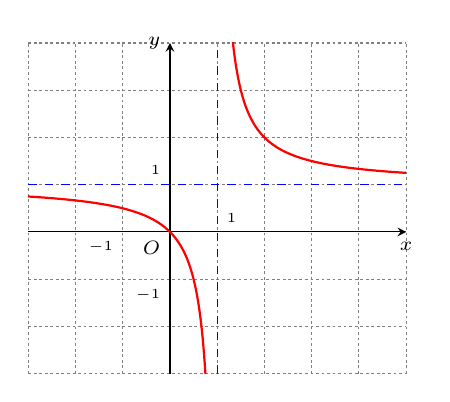
\begin{tikzpicture}[>=stealth,x=1cm,y=1cm,scale=0.6,font=\tiny]
			\def\a{1}
			\def\b{0}
			\def\c{1}
			\def\d{-1}
			\draw[color=gray,dash pattern=on 1pt off 1pt,xstep=1.0cm,ystep=1.0cm] (-3,-3) grid (5,4);
			\draw[->] (-3,0) -- (5,0) node[below] {\scriptsize $x$};
			\draw[->] (0,-3) -- (0,4) node[left] {\scriptsize $y$};
			\draw (0,0)node[below left]{\scriptsize $O$};
			\draw[dashed,blue] (1,-3)--(1,4) (-3,1)--(5,1);
			\fill (-1,0) node[below left]{$-1$};
			\fill (1,0) node[above right]{$1$};
			\fill (0,-1) node[below left]{$-1$};
			\fill (0,1) node[above left]{$1$};
			\clip (-3,-3)rectangle(5,4);
			\pgfmathsetmacro{\can}{-(\d)/(\c)}
			\draw[thick,samples=150,smooth,domain=-5:{\can-.1},red] plot(\x,{(\a*\x+(\b))/(\c*\x+(\d))});
			\draw[thick,samples=150,smooth,domain={\can+.1}:5,red] plot(\x,{(\a*\x+(\b))/(\c*\x+(\d))});
		\end{tikzpicture}
		&
		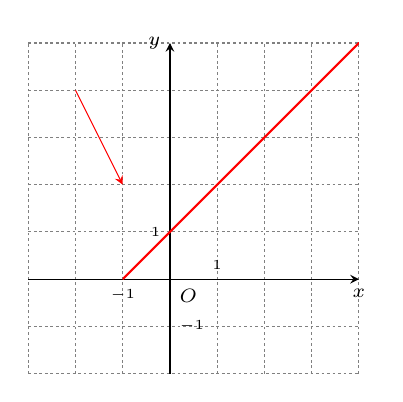
\begin{tikzpicture}[>=stealth,x=1cm,y=1cm,scale=0.6,font=\tiny]
			\def\a{1}
			\def\b{1}
			\draw[color=gray,dash pattern=on 1pt off 1pt,xstep=1.0cm,ystep=1.0cm] (-3,-2) grid (4,5);
			\draw[->] (-3,0) -- (4,0) node[below] {\scriptsize $x$};
			\draw[->] (0,-2) -- (0,5) node[left] {\scriptsize $y$};
			\fill (-1,0) node[below]{$-1$};
			\fill (1,0) node[above]{$1$};
			\fill (0,-1) node[right]{$-1$};
			\fill (0,1) node[left]{$1$};
			\draw (0,0)node[below right]{\scriptsize $O$};
			\draw[red,->] (-2,4)--(-1,2);
			\clip (-1,0)rectangle(4,5);
			\draw[thick,samples=150,smooth,domain=-5:5,red] plot(\x,{\a*\x+(\b)});
		\end{tikzpicture}
		\\
		a) Đồ thị hàm số \break $ f(x)=x^{2}-2x $
		&
		b) Đồ thị hàm số \break $ g(x)=\dfrac{x}{x-1} $
		&
		c) Đồ thị hàm số \break$ h(x)=\heva{&-2x \text{ nếu } x<-1\\&x+1 \text{ nếu }x\geq 1} $
		\\
		&\hspace*{1.5cm}Hình 15& \\
	\end{longtable}
	\loigiai{
		Hàm số liên tục trên tập xác định là $ f(x)=x^{2}-2x $. Vì đồ thị hàm số ở hình \textit{Hình 15a} là một đường liền nét trên mặt phẳng tọa độ. 
	}
\end{bt}

% #715 | Archive/2024/TOAN_11_XE/TOAN_11_XE/data4/11C5/KNTT-5.3.tex | mã gốc 1C3B3-3
\begin{bt}%[Phạm Hoàng Điệp - Dự Án tex  11 mới]%[1C3B3-3]
	Bạn Nam cho rằng: \lq\lq Nếu hàm số $ y=f(x) $ liên tục tại điểm $ x_{0} $, còn hàm số $ y=g(x) $ không liên tục tại $ x_{0} $, thì hàm số $ y=f(x)+g(x) $ không liên tục tại $ x_{0} $\rq\rq. Theo em, ý kiến của bạn Nam đúng hay sai? Giải thích.
	\loigiai{
		Giả sử hàm số $ h(x)=f(x)+g(x) $ là hàm số liên tục tại $ x_{0} $.\\
		Khi đó, hàm số $ g(x)=h(x) -f(x) $ là hiệu của hai hàm số liên tục tại $ x_{0} $ nên hàm số $ g(x) $ là hàm số liên tục tại $ x_{0} $. Điều này mâu thuẫn với giả thiết là $ g(x) $ không liên tục tại $ x_{0} $.	\\
		Vậy ý kiến trên là đúng.
	} 
\end{bt}

% #716 | Archive/2024/TOAN_11_XE/TOAN_11_XE/data4/11C5/KNTT-5.3.tex | mã gốc 1C3B3-4
\begin{bt}%[Phạm Hoàng Điệp - Dự Án tex  11 mới]%[1C3B3-4]
	Xét tính liên tục của mỗi hàm số sau trên tập xác định của hàm số đó
	\begin{enumEX}{3}
		\item $ f(x)=x^{2}+\sin x $.
		\item $ g(x)=x^{4}-x^{2}+\dfrac{6}{x-1} $.
		\item $ h(x)=\dfrac{2x}{x-3}+\dfrac{x-1}{x+4} $.
	\end{enumEX}
	\loigiai{
		\begin{enumerate}
			\item Hàm số $ y=x^{2} $ và hàm số $ y=\sin x $ liên tục trên $ \mathbb{R} $ nên hàm số $ f(x)=x^{2}+\sin x $ là tổng của hai hàm số trên cũng liên tục trên $ \mathbb{R} $.
			\item Tập xác định của hàm số là $ \mathbb{R}\setminus\{1\} $.\\
			Vậy hàm số $ f(x) $ liên tục trên các khoảng $ (-\infty;1) $ và $ (1;+\infty) $.
			\item Tập xác định của hàm số là $ \mathbb{R}\setminus\{-4;3\} $.\\
			Vậy hàm số $ f(x) $ liên tục trên các khoảng $ (-\infty;-4) $; (-4;3) và $ (3;+\infty) $.
		\end{enumerate}
	}
\end{bt}

% #717 | Archive/2024/TOAN_11_XE/TOAN_11_XE/data4/11C5/KNTT-5.3.tex | mã gốc 1C3K3-5
\begin{bt}%[Phạm Hoàng Điệp - Dự Án tex  11 mới]%[1C3K3-5]
	Cho hàm số $ f(x)=\heva{&x^{2}+x+1 &\text{ nếu } x\ne 4\\& 2a+1 &\text{ nếu } x=4.} $
	\begin{enumerate}
		\item Với $ a=0 $, xét lính liên tục của hàm số tại $ x=4 $.
		\item Với giá trị nào của $ a $ thì hàm số liên tục tại $ x=4 $.
		\item Với giá trị nào của $ a $ thì hàm số liên tục trên tập xác định của nó?
	\end{enumerate}
	\loigiai{
		\begin{enumerate}
			\item Hàm số trên là hàm đa thức nên liên tục trên $ \mathbb{R} $.\\
			Ta có $ f(4) =2a+1=1 $ (do $ a=0 $).\\
			$ \displaystyle\lim\limits_{x\to 4}f(x)= \displaystyle\lim\limits_{x\to 4}\left(x^{2}+x+1\right) =4^{2}+4+1 =21$.\\
			Vì  $\displaystyle\lim\limits_{x\to 4}f(x) \ne f(4) $ nên hàm số trên không liên tục tại $ x=4 $ khi $ a=0 $.
			\item Hàm số trên là hàm đa thức nên liên tục trên $ \mathbb{R} $.\\
			Ta có $ f(4) =2a+1 $.\\
			$ \displaystyle\lim\limits_{x\to 4}f(x)= \displaystyle\lim\limits_{x\to 4}\left(x^{2}+x+1\right) =4^{2}+4+1 =21$.\\
			Để hàm số liên tục tại $ x=4 $ thì $ \displaystyle\lim\limits_{x\to 4}f(x) =f(4) \Leftrightarrow 2a+1=21\Leftrightarrow a=10 $.\\
			Vậy $ a=10 $ thì hàm số liên tục tại $ x=4 $.
			\item Tập xác định của hàm số là $ \mathbb{R} $.
			\begin{itemize}
				\item TH1: $ x\ne 4 $, hàm số trên là hàm đa thức nên liên tục trên $ \mathbb{R} $.
				\item TH2: $ x=4 $, hàm số trên là hàm hằng nên liên tục trên $ \mathbb{R} $.
			\end{itemize}
			Vậy hàm số trên liên tục trên $ \mathbb{R} $.
		\end{enumerate}
	}
\end{bt}

% #718 | Archive/2024/TOAN_11_XE/TOAN_11_XE/data4/11C5/KNTT-5.3.tex | mã gốc 1C3B3-4
\begin{bt}%[Phạm Hoàng Điệp - Dự Án tex  11 mới]%[1C3B3-4]
	\immini{Hình bên cạnh biểu thị độ cao $ h $ (m) của một quả bóng được đá lên thời gian $ t $ (s), trong đó $ h(t)= -2t^{2}+8t $.
		\begin{enumerate}
			\item Chứng tỏ hàm số $ h(t) $ liên tục trên tập xác định.
			\item Dựa và đồ thì hãy xác định $ \displaystyle\lim\limits_{t\to 2}\left(-2t^{2}+8t\right) $.
		\end{enumerate}
	}
	{		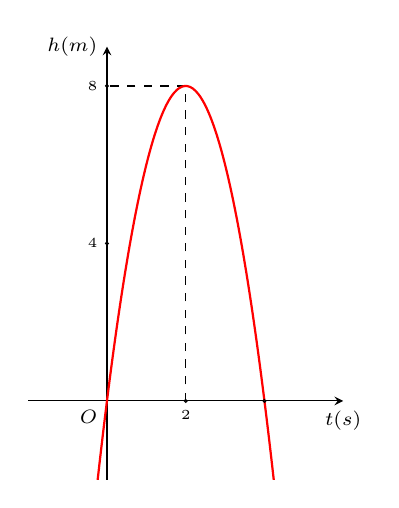
\begin{tikzpicture}[>=stealth,x=1cm,y=1cm,scale=0.5,font=\tiny]
			\def\a{-2}
			\def\b{8}
			\def\c{0}
			\draw[->] (-2,0) -- (6,0) node[below] {\scriptsize $t(s)$};
			\draw[->] (0,-2) -- (0,9) node[left] {\scriptsize $h(m)$};
			\draw (0,0)node[below left]{\scriptsize $O$};
			\fill (0,4) node[left]{$4$};
			\fill (0,8) node[left]{$8$};
			\fill (2,0) node[below]{$2$};
			\draw[dashed] (2,0)--(2,8)--(0,8);
			\pgfmathsetmacro\xdinh{-(\b)/2*(\a)}
			\pgfmathsetmacro\ydinh{(4*(\a)*(\c)-(\b)^2)/(4*(\a))}
			\clip (-2,-2)rectangle(6,9);
			\draw[red,thick,samples=150,smooth,domain=-5:5] plot(\x,{\a*(\x)^2+(\b)*\x+(\c)});
			\foreach \x in {2,4} \draw (\x,0) circle (1pt);
			\foreach \y in {4,8} \draw (0,\y) circle (1pt);
	\end{tikzpicture}}
	\loigiai{
		\begin{enumerate}
			\item Hàm số trên là hàm đa thức nên liên tục trên $ \mathbb{R} $.
			\item Dựa vào đồ thị ta có $  \displaystyle\lim\limits_{t\to 2}\left(-2t^{2}+8t\right) =8 $.
		\end{enumerate}
	}
\end{bt}

% #1004 | Archive/2024/TOAN_11_XE/TOAN_11_XE/data4/11C6/KNTT-6.3.tex | mã gốc 1T3B3-6
\begin{vd}%[Tex hóa SGK CD-CT,T7/22, TVN-019]%[1T3B3-6]
	Công thức $h=-19{,}4\cdot\log\dfrac{P}{P_0}$ là mô hình đơn giản cho phép tính độ cao $h$ so với mặt nước biển của một vị trí trong không trung (tính bằng ki-lô-mét) theo áp suất không khí $P$ tại điểm đó và áp suất $P_0$ của không khí tại mặt nước biển (cùng tính bằng $Pa$ - đơn vị áp suất, đọc là Pascal).
	\begin{center}
		(\textit{Nguồn:}  http://doi.org/10.1007/s40828-020-0111-6)
	\end{center}
	\begin{enumerate}
		\item Nếu áp suất không khí ngoài máy bay bằng $\dfrac{1}{2}P_0$ thì máy bay đang ở độ cao nào?
		\item Áp suất không khí tại đỉnh của ngọn núi A bằng $\dfrac{4}{5}$ lần áp suất không khí tại đỉnh của ngọn núi B. Ngọn núi nào cao hơn và cao hơn bao nhiêu ki-lô-mét? (Làm tròn kết quả đến hàng phần mười.)
	\end{enumerate}
	\loigiai{\begin{enumerate}
			\item Nếu áp suất ở ngoài máy bay là $\dfrac{1}{2}P_0$ thì độ cao của máy bay là $$h=-19{,}4\cdot\log\dfrac{\dfrac{1}{2}P_0}{P_0}=-19{,}4\cdot\log\dfrac{1}{2}\approx5{,}8\text{km}.$$
			\item Gọi áp suất lần lượt của hai ngọn núi A và B là $P_A$, $P_B$. Ta có $P_A=\dfrac{4}{5}P_B$.\\
			Độ cao của núi A và núi B là $\heva{&h_A=-19{,}4\cdot\log\dfrac{P_A}{P_0}\\&h_B=-19{,}4\cdot\log\dfrac{P_B}{P_0}.}$\\
			Ta có
			\begin{eqnarray*}
				h_A&=&-19{,}4\cdot\log\dfrac{P_A}{P_0}=-19{,}4\cdot\log\dfrac{\dfrac{4}{5}P_B}{P_0}\\
				&=&-19{,}4\cdot\left(\log\dfrac{4}{5}+\log\dfrac{P_B}{P_0}\right)=-19{,}4\cdot\log\dfrac{4}{5}+h_B\approx h_B+1{,}9.
			\end{eqnarray*}
			Vậy núi A cao hơn núi B $1{,}9$km.
	\end{enumerate}}
\end{vd}

% #2715 | Archive/SP_KhoLatex/ID6_old/1K5-15-1.tex | mã gốc 1C3B1-2
\begin{bt}%[1C3B1-2]%[Anh Duy]
	Tìm các giới hạn sau
	\begin{enumEX}[a)]{2}
		\item[a)] $\lim \limits_{n \rightarrow+\infty} \dfrac{n^{2}+n+1}{2 n^{2}+1}$.
		\item[b)] $\lim \limits_{n \rightarrow+\infty}\left(\sqrt{n^{2}+2 n}-n\right)$.
	\end{enumEX}
	\loigiai{
		\begin{enumEX}[a)]{1}
			\item $\lim \limits_{n \rightarrow+\infty} \dfrac{n^{2}+n+1}{2 n^{2}+1}=\lim \limits_{n \rightarrow+\infty} \dfrac{1+\dfrac{1}{n}+\dfrac{1}{n^2}}{2+\dfrac{1}{n^2}}=\dfrac{\lim \limits_{n \rightarrow+\infty} \left(1+\dfrac{1}{n}+\dfrac{1}{n^2}\right)}{\lim \limits_{n \rightarrow+\infty} \left(2+\dfrac{1}{n^2}\right)}=\dfrac{1}{2}$.
			\item $\lim \limits_{n \rightarrow+\infty}\left(\sqrt{n^{2}+2 n}-n\right)=\lim \limits_{n \rightarrow+\infty}\dfrac{n^2+2n-n^2}{\sqrt{n^{2}+2 n}+n}=\lim \limits_{n \rightarrow+\infty} \dfrac{2}{\sqrt{1+\dfrac{2}{n}}+1}=\dfrac{2}{\lim \limits_{n \rightarrow+\infty} \left(\sqrt{1+\dfrac{2}{n}}+1\right)}=1$.
		\end{enumEX}
	}
\end{bt}

% #2716 | Archive/SP_KhoLatex/ID6_old/1K5-15-1.tex | mã gốc 1C3B1-2
\begin{bt}%[1C3B1-2]%[Anh Duy]
	Cho hai dãy số không âm $\left(u_{n}\right)$ và $\left(v_{n}\right)$ với $\lim \limits_{n \rightarrow+\infty} u_{n}=2$ và $\lim \limits_{n \rightarrow+\infty} v_{n}=3$. Tìm các giới hạn sau
	\begin{enumEX}[a)]{2}
		\item[a)] $\lim \limits_{n \rightarrow+\infty} \dfrac{u_{n}^{2}}{v_{n}-u_{n}}$;
		\item[b)] $\lim \limits_{n \rightarrow+\infty} \sqrt{u_{n}+2 v_{n}}$.
	\end{enumEX}
	\loigiai{
		\begin{enumEX}[a)]{1}
			\item $\lim \limits_{n \rightarrow+\infty} \dfrac{u_{n}^{2}}{v_{n}-u_{n}} = \dfrac{\lim \limits_{n \rightarrow+\infty} u_{n}^{2}}{\lim \limits_{n \rightarrow+\infty} v_{n}-\lim \limits_{n \rightarrow+\infty} u_{n}} = \dfrac{\left(\lim \limits_{n \rightarrow+\infty} u_{n}\right)^{2}}{\lim \limits_{n \rightarrow+\infty} v_{n}-\lim \limits_{n \rightarrow+\infty} u_{n}}=\dfrac{2^2}{3-2}=4$ ;
			\item $\lim \limits_{n \rightarrow+\infty} \sqrt{u_{n}+2 v_{n}} =  \sqrt{\lim \limits_{n \rightarrow+\infty}  u_{n}+\lim \limits_{n \rightarrow+\infty} 2 v_{n}} =\sqrt{\lim \limits_{n \rightarrow+\infty}  u_{n}+2\lim \limits_{n \rightarrow+\infty}  v_{n}} =\sqrt{2+2\cdot 3}=2\sqrt{2}$.
		\end{enumEX}
	}
\end{bt}

% #2717 | Archive/SP_KhoLatex/ID6_old/1K5-15-1.tex | mã gốc 1C3B1-2
\begin{bt}%[1C3B1-2]%[Anh Duy]
	Tính các giới hạn sau:
	\begin{enumEX}{2}
	\item $\lim \dfrac{2^n+3\cdot 4^n}{4^n-5\cdot 3^n}$.
	\item $T=\lim\dfrac{3\cdot7^n+2\cdot 4^n}{4\cdot 5^n+7^n}$.
	\end{enumEX}
\loigiai{
\begin{enumEX}{1}
	\item $\lim \dfrac{2^n+3\cdot 4^n}{4^n-5\cdot 3^n}=\lim \dfrac{\left(\dfrac {1} {2}\right)^n+3}{1-5\left(\dfrac {3} {4}\right)^n}=3$.
	\item Ta có $T=\lim\dfrac{3\cdot7^n+2\cdot 4^n}{4\cdot 5^n+7^n}=\lim\dfrac{3+2\cdot\left(\dfrac{4}{7}\right)^n}{4\cdot\left(\dfrac{5}{7}\right)^n+1}=3$.
\end{enumEX}
}
\end{bt}

% #2749 | Archive/SP_KhoLatex/ID6_old/1K5-15-4.tex | mã gốc 1T3B1-6
\begin{bt}%[1T3B1-6]
	Tính tổng của các cấp số nhân lùi vô hạn sau
	\begin{listEX}[2]
		\item $-\dfrac{1}{2}+\dfrac{1}{4}-\dfrac{1}{8}+\cdots+\left(-\dfrac{1}{2}\right)^n+\cdots$.
		\item $\dfrac{1}{4}+\dfrac{1}{16}+\dfrac{1}{64}+\cdots+\left(\dfrac{1}{4}\right)^n+\cdots$.
	\end{listEX}
	\loigiai{
		\begin{enumerate}
			\item Tổng trên là tổng của cấp số nhân lùi vô hạn có số hạng đầu $u_1=-\dfrac{1}{2}$ và công bội $q=-\dfrac{1}{2}$ nên 
			\[-\dfrac{1}{2}+\dfrac{1}{4}-\dfrac{1}{8}+\cdots+\left(-\dfrac{1}{2}\right)^n+\cdots=\dfrac{-\dfrac{1}{2}}{1-\left(-\dfrac{1}{2}\right)}=-\dfrac{1}{3}. \]
			\item Tổng trên là tổng của cấp số nhân lùi vô hạn có số hạng đầu $u_1=\dfrac{1}{4}$ và công bội $q=\dfrac{1}{4}$ nên 
			\[\dfrac{1}{4}+\dfrac{1}{16}+\dfrac{1}{64}+\cdots+\left(\dfrac{1}{4}\right)^n+\cdots=\dfrac{\dfrac{1}{4}}{1-\dfrac{1}{4}}=\dfrac{1}{3}. \]
		\end{enumerate}
	}
\end{bt}

% #2750 | Archive/SP_KhoLatex/ID6_old/1K5-15-4.tex | mã gốc 1T3B1-5
\begin{bt}%[1T3B1-5]
	Tính tổng của cấp số nhân lùi vô hạn: $1-\dfrac{1}{4}+\dfrac{1}{16}-\dfrac{1}{64}+\cdots+\left(-\dfrac{1}{4}\right)^n+\cdots$.
	\loigiai{
		Tổng trên là tổng của cấp số nhân lùi vô hạn có số hạng đầu $u_1=1$ và công bội $q=-\dfrac{1}{4}$ nên
		\[ 1-\dfrac{1}{4}+\dfrac{1}{16}-\dfrac{1}{64}+\cdots+\left(-\dfrac{1}{4}\right)^n+\cdots=\dfrac{1}{1-\left(-\dfrac{1}{4}\right)}=\dfrac{4}{5}.\]
	}
\end{bt}

% #2751 | Archive/SP_KhoLatex/ID6_old/1K5-15-4.tex | mã gốc 1T3B1-5
\begin{bt}%[1T3B1-5]
	Biết rằng có thể coi số thập phân vô hạn tuần hoàn $0{,}666 \ldots$ là tổng của một cấp số nhân lùi vô hạn:
	\[ 0{,}666 \ldots=0{,}6+0{,}06+0{,}006+\cdots=0{,}6+0{,}6 \cdot \dfrac{1}{10}+0{,}6 \cdot \dfrac{1}{10^2}+\cdots.
	\]
	Hãy viết $0{,}666 \ldots$ dưới dạng phân số.
	\loigiai{
		Số $0{,}666 \ldots$ là tổng của cấp số nhân lùi vô hạn có số hạng đầu bằng $0{,}6$ và công bội bằng $\dfrac{1}{10}$.\\
		Do đó $0{,}666\ldots=\dfrac{0{,}6}{1-\dfrac{1}{10}}=\dfrac{6}{9}=\dfrac{2}{3}$.
	}
\end{bt}

% #2752 | Archive/SP_KhoLatex/ID6_old/1K5-15-4.tex | mã gốc 1T3B1-5
\begin{bt}%[1T3B1-5]
	Tính tổng của cấp số nhân lùi vô hạn: $1+\dfrac{1}{3}+\left(\dfrac{1}{3}\right)^2+\cdots+\left(\dfrac{1}{3}\right)^n+\cdots$.	
	\loigiai{
		Tổng trên là tổng của cấp số nhân lùi vô hạn có số hạng đầu $u_1=1$ và công bội $q=\dfrac{1}{3}$ nên
		\[ 1+\dfrac{1}{3}+\left(\dfrac{1}{3}\right)^2+\cdots+\left(\dfrac{1}{3}\right)^n+\cdots=\dfrac{1}{1-\dfrac{1}{3}}= \dfrac{3}{2}.\]
	}
\end{bt}

% #2758 | Archive/SP_KhoLatex/ID6_old/1K5-15-5.tex | mã gốc 1T3K1-5
\begin{bt}%[1T3K1-5]
	Từ tờ giấy, cắt một hình tròn bán kính $R$ (cm) như Hình $3a$. Tiếp theo, cắt hai hình~tròn
	\immini{
		bán kính $\dfrac{R}{2}$ rồi chồng lên hình tròn đầu tiên như Hình $3b$. Tiếp theo, cắt bốn hình tròn bán  kính $\dfrac{R}{4}$ 
		rồi chồng lên các hình trước như Hình $3c$. Cứ thế tiếp tục mãi. Tính tổng diện tích của các hình tròn.
	}{
		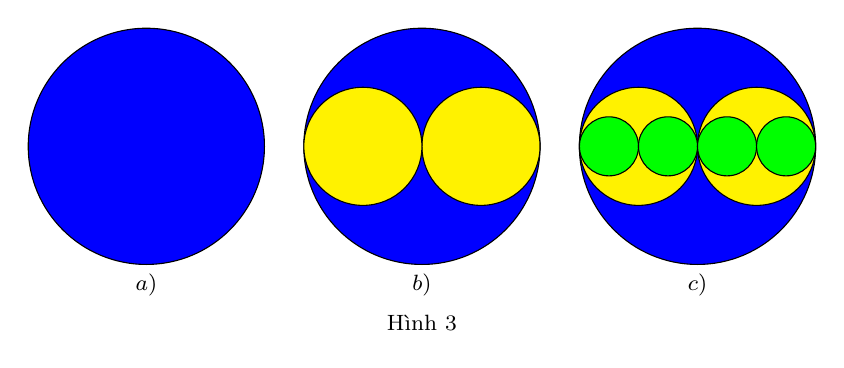
\begin{tikzpicture}[>=stealth,line join=round,line cap=round,font=\footnotesize,scale=1,declare function={r=1.5;}]
			\begin{scope}
				\draw[fill=blue] (0,0)circle(r);
				\path (0,-r) node[below]{$a)$};
			\end{scope}
			\begin{scope}[xshift={3.5cm}]
				\draw[fill=blue] (0,0)circle(r);
				\draw[fill=yellow] (r/2,0)circle(r/2);
				\draw[fill=yellow] (-r/2,0)circle(r/2);
				\path (0,-r) node[below]{$b)$};
			\end{scope}
			\begin{scope}[xshift={7cm}]
				\draw[fill=blue] (0,0)circle(r);
				\draw[fill=yellow] (r/2,0)circle(r/2);
				\draw[fill=yellow] (-r/2,0)circle(r/2);
				\foreach \i in {0,1,2,3}
				\draw[fill=green,shift={(r/2*\i,0)}] (-3*r/4,0)circle(r/4);
				\path (0,-r) node[below]{$c)$};
			\end{scope}
			\path (current bounding box.south) node[below]{Hình $3$};
		\end{tikzpicture}
	}
	\loigiai{
		Diện tích của các hình tròn trong các lần cắt là
		\begin{enumerate}
			\item Lần thứ 1: $S_1=\pi R^2$.
			\item  Lần thứ 2: $S_2=2\cdot \pi \left(\dfrac{R}{2}\right)^2= \dfrac{\pi R^2}{2}$.
			\item  Lần thứ 3: $S_2=4\cdot \pi \left(\dfrac{R}{4}\right)^2= \dfrac{\pi R^2}{2^2}$.	
			\item Lần thứ $n$: $S_n= \dfrac{\pi R^2}{2^{n-1}}$.
		\end{enumerate}
		Do đó  diện tích các hình tròn lập thành một cấp số nhân lùi vô hạn có số hạng đầu $S_1=\pi R^2$ và công bội $q=\dfrac{1}{2}$ nên tổng diện tích các hình tròn là 
		\[ S_1+S_2+\cdots=\dfrac{\pi R^2}{1-\dfrac{1}{2}}=2\pi R^2. \]
	}
\end{bt}

% #2759 | Archive/SP_KhoLatex/ID6_old/1K5-15-5.tex | mã gốc 1T3K1-5
\begin{bt}%[1T3K1-5]
	\immini{
		Từ hình vuông đầu tiên có cạnh bằng $1$ (đơn vị độ dài), nối các trung điểm của bốn cạnh để có hình vuông thứ hai. Tiếp tục nối các trung điểm của bốn cạnh của hình vuông thứ hai để được hình vuông thứ ba. Cứ tiếp tục làm như thế, nhận được một dãy hình vuông (xem Hình $5$).
	}{\hspace*{.5cm}
		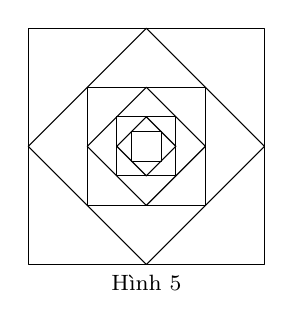
\begin{tikzpicture}[>=stealth,line join=round,line cap=round,font=\footnotesize,scale=1,declare function={a=3;}]
			\foreach \i in {1,2,...,7}{
				\pgfmathsetmacro\r{a*(sin(45))^(\i-1)}
				\pgfmathsetmacro{\j}{int(mod(\i,2))}
				\ifnum \j=1
				\draw (-\r/2,-\r/2) rectangle (\r/2,\r/2);
				\else
				\draw[rotate=45] (-\r/2,-\r/2) rectangle (\r/2,\r/2);
				\fi
			}
			\path (current bounding box.south) node[below]{Hình $5$};
		\end{tikzpicture}\hspace*{1cm}
	}
	\begin{enumerate}
		\item Kí hiệu $a_n$ là diện tích của hình vuông thứ $n$ và $S_n$ là tổng diện tích của $n$ hình vuông đầu tiên. Viết công thức tính $a_n$, $S_n$ ($n=1,2,3, \ldots$) và tìm $\lim S_n$ (giới hạn này nếu có được gọi là tổng diện tích của các hình vuông).
		\item Kí hiệu $p_n$ là chu vi của hình vuông thứ $n$ và $Q_n$ là tổng chu vi của $n$ hình vuông đầu tiên. Viết công thức tính $p_n$ và $Q_n$ $(n=1,2,3, \ldots)$ và tìm $\lim Q_n$ (giới hạn này nếu có được gọi là tổng chu vi của các hình vuông).
	\end{enumerate}
	\loigiai{
		\begin{enumerate}
			\item Ta có hình vuông thứ nhất có cạnh bằng $1$,
			hình vuông thứ hai có cạnh bằng $\dfrac{\sqrt{2}}{2}$.\\
			Hình vuông thứ ba có cạnh bằng $\dfrac{1}{2}$.\\
			Suy ra	hình vuông thứ $n$ có cạnh bằng $\left(\dfrac{\sqrt{2}}{2}\right)^{n-1}$.\\
			Diện tích của hình vuông thứ $n$ là $a_n=\left(\dfrac{\sqrt{2}}{2}\right)^{n-1}\cdot \left(\dfrac{\sqrt{2}}{2}\right)^{n-1}=\left(\dfrac{1}{2}\right)^{n-1}$.\\
			Tổng diện tích của $n$ hình vuông đầu tiên là tổng của cấp số nhân có  số hạng đầu $a_1=1$ và công bội $q=\dfrac{1}{2}$ nên
			\[ S_n=\dfrac{a_1\left(1-q^n\right)}{1-q}=\dfrac{1-\left(\dfrac{1}{2}\right)^n}{1-\dfrac{1}{2}}=2\left[1-\left(\dfrac{1}{2}\right)^n\right].\]
			$\lim S_n=\lim 2\left[1-\left(\dfrac{1}{2}\right)^n\right]=2 \left[\lim 1-\lim \left(\dfrac{1}{2}\right)^n\right]=2 $.
			\item Hình vuông thứ nhất có chu vi bằng $4$, hình vuông thứ $2$ có chu vi là $2\sqrt{2}$, hình vuông thứ $3$ có chu vi là $2$.\\
			Suy ra hình vuông thứ $n$ có chu vi bằng $p_n=4\cdot \left(\dfrac{\sqrt{2}}{2}\right)^{n-1}$.
			Tổng chu vi của $n$ hình vuông đầu tiên là tổng của cấp số nhân có  số hạng đầu $p_1=4$ và công bội $q=\dfrac{\sqrt{2}}{2}$ nên 
			\[ Q_n=\dfrac{p_1\left(1-q^n\right)}{1-q}=\dfrac{4\left(1-\left(\dfrac{\sqrt{2}}{2}\right)^n\right)}{1-\dfrac{\sqrt{2}}{2}}=\left(8+4\sqrt{2}\right)\left[1-\left(\dfrac{\sqrt{2}}{2}\right)^n\right].\]
			$\lim Q_n=\left(8+4\sqrt{2}\right)\lim \left[1-\left(\dfrac{\sqrt{2}}{2}\right)^n\right]=\left(8+4\sqrt{2}\right)\left(1-0\right)=8+4\sqrt{2}$.
		\end{enumerate}	
	}
\end{bt}

% #2760 | Archive/SP_KhoLatex/ID6_old/1K5-15-5.tex | mã gốc 1T3K1-4
\begin{bt}%[1T3K1-4]
	Xét quá trình tạo ra hình có chu vi vô cực và diện tích bằng $0$ như sau:\\ Bắt đầu bằng một hình vuông $H_0$ cạnh bằng 1 đơn vị độ dài (xem Hình $6a$). Chia hình vuông $H_0$ thành chín hình vuông bằng nhau, bỏ đi bốn hình vuông, nhận được hình $H_1$ (xem Hình $6b$). Tiếp theo, chia mỗi hình vuông của $H_1$ thành chín hình vuông, rồi bỏ đi bốn hình vuông, nhận được hình $H_2$ (xem Hình $6c$). Tiếp tục quá trình này, ta nhận được một dãy hình $H_n$ $(n=1,2,3,\ldots)$.	
	\\[1mm]
	\centerline{
		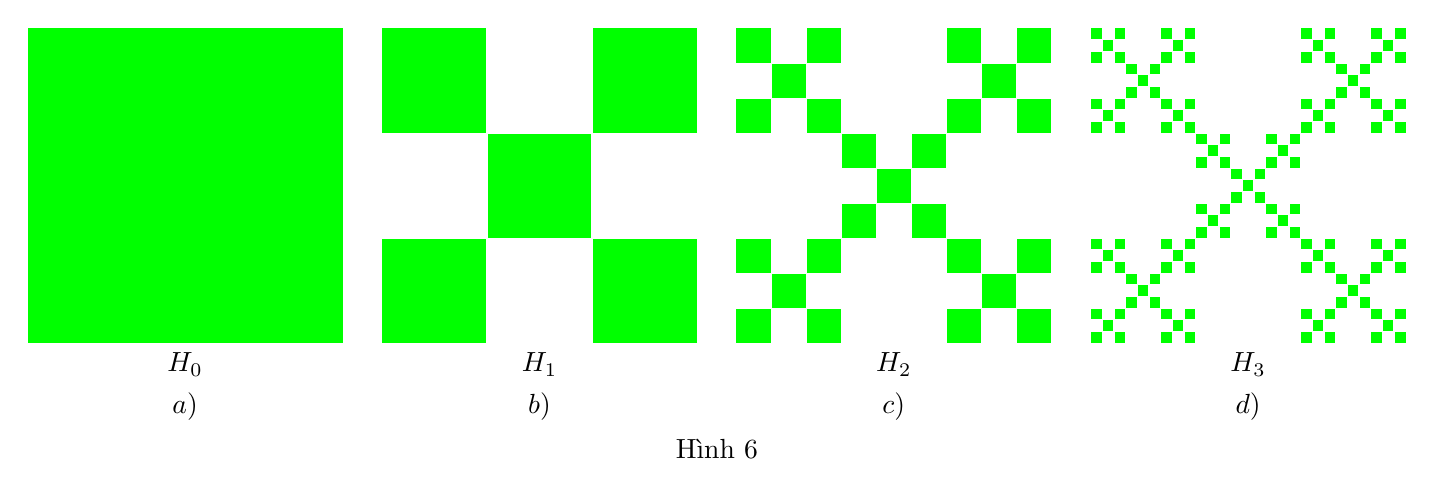
\begin{tikzpicture}% Muốn vẽ hình Hn thì dùng \hv{n}
			\def\a{2}
			\pgfmathsetmacro\sh{2*\a *sqrt(2)/3}
			\def\hv#1{
				\ifnum#1>0
				\draw[white,fill=white] 
				(-\a/3,\a/3) rectangle (\a/3,\a)
				(-\a/3,-\a/3) rectangle (-\a,\a/3)
				(-\a/3,-\a/3) rectangle (\a/3,-\a)
				(\a/3,-\a/3) rectangle (\a,\a/3)
				;
				\pgfmathtruncatemacro{\k}{#1-1}
				\begin{scope}[scale=1/3]\hv{\k}\end{scope}
				\begin{scope}[shift={(45:\sh)},scale=1/3]\hv{\k}\end{scope}
				\begin{scope}[shift={(135:\sh)},scale=1/3]\hv{\k}\end{scope}
				\begin{scope}[shift={(225:\sh)},scale=1/3]\hv{\k}\end{scope}
				\begin{scope}[shift={(315:\sh)},scale=1/3]\hv{\k}\end{scope}
				\fi
			}
			\begin{scope}
				\fill[green] (-\a,-\a) rectangle (\a,\a);
				\hv{0}
				\path (0,-\a)node[below]{$H_0$}
				node[below=.5cm]{$a)$};
			\end{scope}
			\begin{scope}[xshift=4.5cm]
				\fill[green] (-\a,-\a) rectangle (\a,\a);
				\hv{1}
				\path (0,-\a)node[below]{$H_1$}
				node[below=.5cm]{$b)$};
			\end{scope}
			\begin{scope}[xshift=9cm]
				\fill[green] (-\a,-\a) rectangle (\a,\a);
				\hv{2}
				\path (0,-\a)node[below]{$H_2$}
				node[below=.5cm]{$c)$};
			\end{scope}
			\begin{scope}[xshift=13.5cm]
				\fill[green] (-\a,-\a) rectangle (\a,\a);
				\hv{3}
				\path (0,-\a)node[below]{$H_3$}
				node[below=.5cm]{$d)$};
			\end{scope}
			\path (current bounding box.south) node[below]{Hình $6$};
		\end{tikzpicture}
	}
	Ta có: $H_1$ có $5$ hình vuông, mỗi hình vuông có cạnh bằng $\dfrac{1}{3}$;\\
	{\color{white}{Ta có: }}$H_2$ có $5\cdot5=5^2$ hình vuông, mỗi hình vuông có cạnh bằng $\dfrac{1}{3} \cdot \dfrac{1}{3}=\dfrac{1}{3^2}; \ldots$.\\
	Từ đó, nhận được $H_n$ có $5^n$ hình vuông, mỗi hình vuông có cạnh bằng $\dfrac{1}{3^n}$.
	\begin{enumerate}
		\item Tính diện tích $S_n$ của $H_n$ và tính $\lim S_n$.
		\item Tính chu vi $p_n$ của $H_n$ và tính $\lim p_n$.
	\end{enumerate}
	(Quá trình trên tạo nên một hình, gọi là một fractal, được coi là có diện tích $\lim S_n$ và chu vi $\lim p_n$).
	\loigiai{
		\begin{enumerate}
			\item Hình vuông $H_1$ có diện tích $S_1=5\cdot \left(\dfrac{1}{3}\right)^2=\dfrac{5}{9}$.\\
			Hình vuông $H_2$ có diện tích $S_2=5^2\cdot \left(\dfrac{1}{3^2}\right)^2=\left(\dfrac{5}{9}\right)^2$.\\
			Hình vuông $H_n$ có diện tích $S_n=5^n\cdot \left(\dfrac{1}{3^n}\right)^2=\left(\dfrac{5}{9}\right)^n$.\\
			$\lim S_n=\lim \left(\dfrac{5}{9}\right)^n=0$.
			\item Hình vuông $H_1$ có chu vi $p_1=5\cdot 4\cdot  \dfrac{1}{3}=4\cdot \dfrac{5}{3}$.\\
			Hình vuông $H_2$ có chu vi $p_2=5^2\cdot4\cdot \dfrac{1}{3^2}=4\cdot \left(\dfrac{5}{3}\right)^2$.\\
			Hình vuông $H_n$ có diện tích $p_n=5^n\cdot4\cdot  \dfrac{1}{3^n}=4\cdot \left(\dfrac{5}{3}\right)^n$.\\
			$\lim p_n=\lim 4\cdot \left(\dfrac{5}{3}\right)^n=+\infty$.
		\end{enumerate}
	}
\end{bt}

% #2761 | Archive/SP_KhoLatex/ID6_old/1K5-15-5.tex | mã gốc 1T3K1-5
\begin{bt}%[1T3K1-5]
	\immini{Cho tam giác đều có cạnh bằng $a$, gọi là tam giác $H_1$. Nối các trung điểm của $H_1$ để tạo thành tam giác $\mathrm{H}_2$. Tiếp theo, nối các trung điểm của $\mathrm{H}_2$ để tạo thành tam giác $\mathrm{H}_3$ (Hình bên). Cứ tiếp tục như vậy, nhận được dãy tam giác $H_1, H_2, H_3, \ldots$\\
		Tính tổng chu vi và tổng diện tích các tam giác của dãy.}{
		\begin{tikzpicture}[scale=1, font=\footnotesize, line join=round, line cap=round, >=stealth]
			(0,0) coordinate (A)	
			(4,0) coordinate (B)	
			(2,2.8284) coordinate (C)
			\draw (A)--(B)--(C)--cycle;
			\coordinate (I) at ($(A)!0.5!(B)$);
			\coordinate (J) at ($(B)!0.5!(C)$);
			\coordinate (K) at ($(C)!0.5!(A)$);
			\draw (I)--(J)--(K)--cycle;
			\coordinate (H) at ($(I)!0.5!(J)$);
			\coordinate (G) at ($(J)!0.5!(K)$);
			\coordinate (F) at ($(K)!0.5!(I)$);
			\draw (H)--(G)--(F)--cycle;
			\coordinate (X) at ($(H)!0.5!(G)$);
			\coordinate (Y) at ($(G)!0.5!(F)$);
			\coordinate (Z) at ($(F)!0.5!(H)$);
			\draw (X)--(Y)--(Z)--cycle;
			\draw[dashed] (2,2.8284)--(3.3,1.45)node[above right]{$a$}--(4,0);
		\end{tikzpicture}
	}
	\loigiai{
		Gọi $S_i$ và $C_i$ ($i=1,2,\ldots$) lần lượt là diện tích và chu vi của tam giác $H_i$, $i=1,2,\ldots $.\\
		Khi đó ta có
		\begin{itemize}
			\item[$\bullet$] $S_1=\dfrac{a^2\sqrt{3}}{4};S_2=\left(\dfrac{a}{2}\right)^2\dfrac{\sqrt{3}}{4}=\dfrac{a^2\sqrt{3}}{16}=\dfrac{S_1}{4};S_3=\dfrac{1}{4}S_2,\ldots $.\\
			Do đó $(S_n)$ là một cấp số nhân lùi vô hạn với $S_1=\dfrac{a^2\sqrt{3}}{4}$ và $q_1=\dfrac{1}{4}$.\\
			Tổng diện tích $S=S_1+S_2+\cdots =\dfrac{S_1}{1-q_1}=\dfrac{a^2\sqrt{3}}{3}$.
			\item[$\bullet$] $C_1=3a; C_2=\dfrac{3a}{2}=\dfrac{1}{2}C_1,\ldots$\\
			Do đó $(C_n)$ là một cấp số nhân lùi vô hạn với $C_1=3a;q_2=\dfrac{1}{2}$.\\
			Tổng chu vi là $C=C_1+C_2+\cdots =\dfrac{C_1}{1-q_2}=6a$.
		\end{itemize}
	}	
\end{bt}

% #3812 | Archive/SP_KhoLatex/ID6_old/1-GK1-CTST-De12-NH23-24.tex | mã gốc 1T3B3-5
\begin{bt}%[1T3B3-5]
	Tìm tất cả các giá trị của tham số thực $m$ sao cho hàm số $f(x)=\heva{& \sqrt{x}-m & \text { khi } x \geq 0 \\ &m x+2 & \text { khi } x<0}$ liên tục trên $\mathbb{R}$.
	\loigiai{
	Trên khoảng $(0 ;+\infty)$ hàm số $f(x)=2 \sqrt{x}-m$ là hàm số liên tục.\\
	Trên khoảng $(-\infty ; 0)$ hàm số $f(x)=m x+2$ là hàm số liên tục.\\
	Ta có $\displaystyle\lim _{x \rightarrow 0^{+}} f(x)=\displaystyle\lim _{x \rightarrow 0^{+}}(2 \sqrt{x}-m)=-m=f(0)$ và $\displaystyle\lim _{x \rightarrow 0^{-}} f(x)=\displaystyle\lim _{x \rightarrow 0^{-}}(m x+2)=2$.\\
	Hàm số $f(x)$ liên tục trên $\mathbb{R} \Leftrightarrow \displaystyle\lim _{x \rightarrow 0^{+}} f(x)=\displaystyle\lim _{x \rightarrow 0^{-}} f(x)=f(0) \Leftrightarrow-m=2 \Leftrightarrow m=-2$.
	}
\end{bt}
